\documentclass[a4paper,14pt]{extarticle}

% Путь до папки с общими шаблонами
\newcommand{\pathToCommonFolder}{/home/denilai/Documents/repos/latex/Common}
% Название работы в титуле
\newcommand{\workname}{Отчет по практической работе №1}
% Название дисциплины в титуле
\newcommand{\discipline}{Основы сетевых технологий}
% Название кафедры в титуле
\newcommand{\kafedra}{Кафедра вычислительной техники}
% Тема работы в титуле
\newcommand{\theme}{Базовая настройка коммутатора}
% Должность преподавателя в титуле
\newcommand{\rang}{cтарший преподаватель кафедры ВТ}
% ФИО преподавателя в титуле
\newcommand{\teacherfio}{Ю.~М.Скрябин}
\newcommand{\studentfio}{К.~Ю.~Денисов}
\newcommand{\signature}{\pathToCommonFolder/denisov-signature}

\newcommand{\pt}{PacketTracer\copyright}

\usepackage{tabularx}

\newcommand{\router}{R1\_DENISOV~}
\newcommand{\switch}{S1~}



\usepackage{booktabs}
\newcolumntype{b}{X}
\newcolumntype{s}{>{\hsize=.5\hsize}X}
\newcommand{\heading}[1]{\multicolumn{1}{|c|}{#1}}

% установка размера шрифта для всего документа
%\fontsize{20pt}{18pt}\selectfont
\usepackage{extsizes} % Возможность сделать 14-й шрифт

% Вставка заготовки преамбулы
% Этот шаблон документа разработан в 2014 году
% Данилом Фёдоровых (danil@fedorovykh.ru) 
% для использования в курсе 
% <<Документы и презентации в \LaTeX>>, записанном НИУ ВШЭ
% для Coursera.org: http://coursera.org/course/latex .
% Исходная версия шаблона --- 
% https://www.writelatex.com/coursera/latex/5.3

% В этом документе преамбула

% Для корректного использования русских символов в формулах
% пакеты hyperref и настройки, связанные с ним, стоит загуржать
% перед загрузкой пакета mathtext



% поддержка русских букв
% кодировка шрифта
%\usepackage[T2A]{fontenc} 
\usepackage{pscyr}

% использование ненумеровонного абзаца с добавлением его в содержаниеl

\newcommand{\anonsection}[1]{\section*{#1}\addcontentsline{toc}{section}{#1}}
\newcommand{\sectionunderl}[1]{\section*{\underline{#1}}}


% настройка окружения enumerate
\usepackage{enumitem}
\setlist{noitemsep}
\setlist[enumerate]{labelsep=*, leftmargin=1.5pc}

\usepackage{hyperref}

% сначала ставить \usepackage{extsizes} % Возможность сделать 14-й шрифт
% для корректной установки полей вставлять преамбулу следует в последнюю очередь (но перед дерективой замены \rmdefault)
\usepackage[top=20mm,bottom=25mm,left=35mm,right=20mm]{geometry} % Простой способ задавать поля

\hypersetup{				% Гиперссылки
	unicode=true,           % русские буквы в раздела PDF
	pdftitle={Заголовок},   % Заголовок
	pdfauthor={Автор},      % Автор
	pdfsubject={Тема},      % Тема
	pdfcreator={Создатель}, % Создатель
	pdfproducer={Производитель}, % Производитель
	pdfkeywords={keyword1} {key2} {key3}, % Ключевые слова
	colorlinks=true,       	% false: ссылки в рамках; true: цветные ссылки
	linkcolor=red,          % внутренние ссылки
	citecolor=black,        % на библиографию
	filecolor=magenta,      % на файлы
	urlcolor=blue           % на URL
}

%%% Работа с русским языком
\usepackage{cmap}					% поиск в PDF
\usepackage{mathtext} 				% русские буквы в формулах
\usepackage[T2A]{fontenc}			% кодировка
\usepackage[utf8]{inputenc}			% кодировка исходного текста
\usepackage[english,russian]{babel}	% локализация и переносы
\usepackage{indentfirst}
\frenchspacing

%для изменения названия списка иллюстраций
\usepackage{tocloft}


\renewcommand{\epsilon}{\ensuremath{\varepsilon}}
\renewcommand{\phi}{\ensuremath{\varphi}}
\renewcommand{\kappa}{\ensuremath{\varkappa}}
\renewcommand{\le}{\ensuremath{\leqslant}}
\renewcommand{\leq}{\ensuremath{\leqslant}}
\renewcommand{\ge}{\ensuremath{\geqslant}}
\renewcommand{\geq}{\ensuremath{\geqslant}}
\renewcommand{\emptyset}{\varnothing}

% Изменения параметров списка иллюстраций
\renewcommand{\cftfigfont}{Рисунок } % добавляем везде "Рисунок" перед номером
\addto\captionsrussian{\renewcommand\listfigurename{Список иллюстративного материала}}

\newcommand{\tm}{\texttrademark\ }
\newcommand{\reg}{\textregistered\ }


%%% Дополнительная работа с математикой
\usepackage{amsmath,amsfonts,amssymb,amsthm,mathtools} % AMS
\usepackage{icomma} % "Умная" запятая: $0,2$ --- число, $0, 2$ --- перечисление

%% Номера формул
%\mathtoolsset{showonlyrefs=true} % Показывать номера только у тех формул, на которые есть \eqref{} в тексте.
%\usepackage{leqno} % Нумереация формул слева

%% Свои команды
\DeclareMathOperator{\sgn}{\mathop{sgn}}

%% Перенос знаков в формулах (по Львовскому)
\newcommand*{\hm}[1]{#1\nobreak\discretionary{}
{\hbox{$\mathsurround=0pt #1$}}{}}


% отступ для первого абзаца главы или параграфа
%\usepackage{indentfirst}

%%% Работа с картинками
\usepackage{graphicx}  % Для вставки рисунков
\graphicspath{{images/}{screnshots/}}  % папки с картинками
\DeclareGraphicsExtensions{.pdf,.png,.jpg}
\setlength\fboxsep{3pt} % Отступ рамки \fbox{} от рисунка
\setlength\fboxrule{1pt} % Толщина линий рамки \fbox{}
\usepackage{wrapfig} % Обтекание рисунков текстом

%%% Работа с таблицами
\usepackage{array,tabularx,tabulary,booktabs} % Дополнительная работа с таблицами
\usepackage{longtable}  % Длинные таблицы
\usepackage{multirow} % Слияние строк в таблице

%%% Теоремы
\theoremstyle{plain} % Это стиль по умолчанию, его можно не переопределять.
\newtheorem{theorem}{Теорема}[section]
\newtheorem{proposition}[theorem]{Утверждение}

\theoremstyle{plain} % Это стиль по умолчанию, его можно не переопределять.
\newtheorem{work}{Практическая работа}[part]


 
 
\theoremstyle{definition} % "Определение"
\newtheorem{corollary}{Следствие}[theorem]
\newtheorem{problem}{Задача}[section]
 
\theoremstyle{remark} % "Примечание"
\newtheorem*{nonum}{Решение}



%%% Программирование
\usepackage{etoolbox} % логические операторы

%%% Страница

%	\usepackage{fancyhdr} % Колонтитулы
% 	\pagestyle{fancy}
%   \renewcommand{\headrulewidth}{0pt}  % Толщина линейки, отчеркивающей верхний колонтитул
% 	\lfoot{Нижний левый}
% 	\rfoot{Нижний правый}
% 	\rhead{Верхний правый}
% 	\chead{Верхний в центре}
% 	\lhead{Верхний левый}
%	\cfoot{Нижний в центре} % По умолчанию здесь номер страницы

\usepackage{setspace} % Интерлиньяж
\onehalfspacing % Интерлиньяж 1.5
%\doublespacing % Интерлиньяж 2
%\singlespacing % Интерлиньяж 1

\usepackage{lastpage} % Узнать, сколько всего страниц в документе.

\usepackage{soul} % Модификаторы начертания


\usepackage[usenames,dvipsnames,svgnames,table,rgb]{xcolor}


\usepackage{csquotes} % Еще инструменты для ссылок

%\usepackage[style=authoryear,maxcitenames=2,backend=biber,sorting=nty]{biblatex}

\usepackage{multicol} % Несколько колонок

\usepackage{tikz} % Работа с графикой
\usepackage{pgfplots}
\usepackage{pgfplotstable}

% модуль для вставки рыбы
\usepackage{blindtext}

\usepackage{listings}
\usepackage{color}


% для поворота отдельной страницы. Использовать окружение \landscape
\usepackage{pdflscape} 
\usepackage{rotating} 


\definecolor{mygreen}{rgb}{0,0.6,0}
\definecolor{mygray}{rgb}{0.5,0.5,0.5}
\definecolor{mymauve}{rgb}{0.58,0,0.82}


% пример импорта файла
%\lstinputlisting{/home/denilai/repomy/conf/distributions}

\lstset{
	language=Python,
	basicstyle=\footnotesize,        % the size of the fonts that are used for the code
	numbers=left,                    % where to put the line-numbers; possible values are (none, left, right)
	numbersep=5pt,                   % how far the line-numbers are from the code
	numberstyle=\tiny\color{mygray}, % the style that is used for the line-numbers
	stepnumber=2,                    % the step between two line-numbers. If it's 1, each line will be numbered
	% Tab - 2 пробела
	tabsize=2,    
	% Автоматический перенос строк
	breaklines=true,
	frame=single,
	breakatwhitespace=true,
	title=\lstname 
}



\author{Кирилл Денисов ИВБО-02-19}
\title{Практическая работа №1\\Вариант 6}
\date{\today}

\renewcommand{\withouttheme}{1}

% установка полуторного интервала
% \usepackage{setspace}  
% \onehalfspacing

% использовать Times New Roman
\renewcommand{\rmdefault}{ftm}


\begin{document}
	%\thispagestyle{empty}
	% Вставка первого титульного листа
	%%\newcommand{\withouttheme}{} добавить эту переменную для определения, нужна ли тема
%     {} - нужна
%    {1} - не нужна

%\newcommand{\withoutsubmissiondate}{} добавить эту переменную для определения, нужен ли срок предоставления отчета
%     {} - нужен
%    {1} - не нужен
\begin{center}
	\begin{figure}[h!]
		\begin{center}
		
\includegraphics[width=0.17\linewidth]{\pathToCommonFolder/gerb}
		%\caption{}\label{pic:first}
		%	\vspace{5ex}
		\end{center}	
	\end{figure}
 	\small	МИНОБРНАУКИ РОССИИ \\
	Федеральное государственное бюджетное образовательное учреждение\\
						высшего профессионального образования\\
\normalsize					
\textbf{«МИРЭА – Российский технологический университет»\\
						РТУ МИРЭА}\\
						\noindent\rule{1\linewidth}{1pt}\\
       Институт информационных технологий\\ %\vspace{2ex}
					\kafedra\\
		\vspace{3ex}
			\large \textbf{\workname}  \\
		%\vspace{1ex}
						по дисциплине\\ «\discipline» \\
		\vspace{3ex}
		\if \withouttheme
			\textbf{Тема работы:}\\ <<\theme>>
		\fi
\vspace{3ex}
\small
\begin{table}[h!]
\begin{tabular}{p{0.14\linewidth}p{0.38\linewidth}p{0.25\linewidth}p{0.2\linewidth}}
	\textbf{Выполнил:} & студент группы ИВБО-02-19 & \studentfio &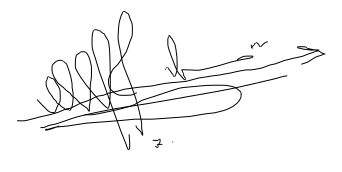
\includegraphics[width=0.8\linewidth]{\signature}\\ \\
	\textbf{Принял:} & \rang & \teacherfio 
\end{tabular}
\end{table}
\end{center}

\begin{flushleft}
	\begin{tabular}{p{0.25\linewidth}l}

		Работа выполена & <<\noindent\rule{2em}{1pt}>>
		                    \noindent\rule{5em}{1pt} 202\noindent\rule{1em}{1pt} \\

		<<Зачтено>> & <<\noindent\rule{2em}{1pt}>>
		\noindent\rule{5em}{1pt} 202\noindent\rule{1em}{1pt} \\

	\end{tabular}
\end{flushleft}

\normalsize
\begin{center}	
\vfill 
Москва 2021
\end{center}

	\newpage
	%\tableofcontents
	\newpage
	%\listoftables
\maketitle


\begin{table}[htbp]
	\begin{center}
		\caption{Таблица адресации}
		\begin{tabular}{|l|l|l|}
			\hline\
			\textbf{Устройство}  & \textbf{Интерфейс} & \textbf{IP-адрес} \\ \hline
			\multirow{3}{*}{\router} & \multirow{3}{*}{VLAN 6}    & 192.168.1.8 /24 \\\cline{3-3}
			& & 2001:db8:acad::2 /64 \\\cline{3-3}
			& & fe80::2 \\\hline
			\multirow{3}{*}{PC-A}   & 	\multirow{3}{*}{NIC}    & 192.168.1.16 /24  \\\cline{3-3}
			                        &                           & 2001:db8:acad::3 /64\\\cline{3-3}
			                        &  &fe80::3\\\hline
		\end{tabular}
		\label{tab:adress}
	\end{center}
\end{table}

\mypart{Создание сети и проверка настроек коммутатора по умолчанию}

\step{Создайте сеть согласно топологии}
Соединили устройства согласно предложенной топологии. Установили консольное подключение к коммутатору, необходимое для первичной настройки устройства, когда конфигурация соединений по SSH и Telnet не настроена (см. рисунок \ref{fig:topology}).

% TODO: \usepackage{graphicx} required
\begin{figure}[h!]
	\centering
	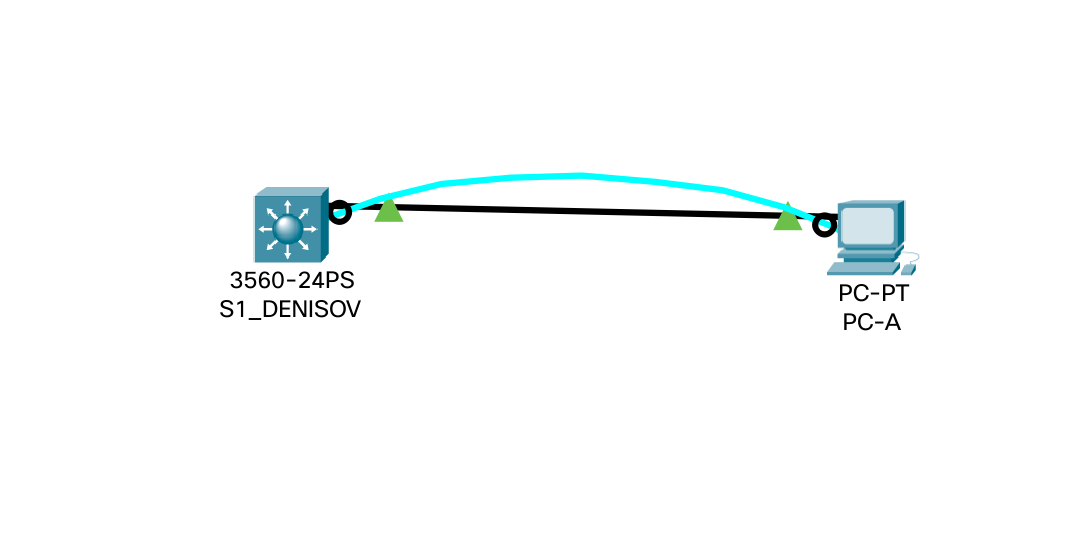
\includegraphics[width=0.6\linewidth]{images/topology}
	\caption{Топология сети}
	\label{fig:topology}
\end{figure}

\step{Проверьте настройки коммутатора по умолчанию}{
Проверим, что коммутатор не имеет файла конфигурации, сохраненного в энергонезависимой
памяти (NVRAM).
На коммутаторе присутствуют 24 интерфейса FastEthernet, 2 интерфейса GigabyteEthernet, 16 линий vty. В исходном состоянии VLAN 1 не настроен, адреса не заданы.

Изучим сведения о OS коммутатора с помощью команды \textit{\# show version}.
Чтобы включить интерфейс необходимо ввести команду \textit{no shutdown}, находясь в режиме конфигурации данного интерфейса.

По умолчанию имя vlan 1 --- Vlan 1.

Изучив флеш-память, видим, что образу Cisco OS присвоено имя c3560-advipservicesk9-mz.122-37.SE1.}

\mypart{Настройка базовых параметров сетевых устройств}

\step{Настройте базовые параметры коммутатора}
{
Введем следующие команды в консоль коммутатора, находясь в режиме конфигурации. 

\begin{lstlisting}
	no ip domain-lookup
	hostname S1_DENISOV
	service password-encryption
	enable secret class
	banner motd #
	Unauthorized access is strictly prohibited. #
\end{lstlisting}
}

Назначим адреса IPV4 и IPV6 VLAN 6 коммутатора согласно заданию. Чтобы включить поддержку IP6 на коммутаторе 3560, необходимо выполнить следующие действия. 

\begin{lstlisting}
	conf t
	sdm prefer dual-ipv4-and-ipv6 default
	wr
	reload
	conf t
	ipv6 unicast-routing
\end{lstlisting}

Ассоциируем все порты коммутатора с данным виртуальным интерфейсом, использовав команды \textit{switchport mode access} и \textit{switchport access vlan6}? находясь в режиме конфигурации выбранных интерфейсов, активируем интерфейс (см. рисунки \ref{fig:vlan-brief} и \ref{fig:run-conf-vlan}).

% TODO: \usepackage{graphicx} required
\begin{figure}[h!]
	\centering
	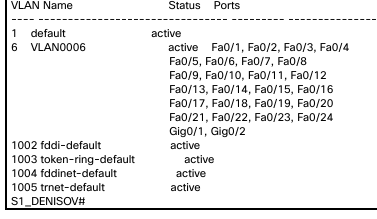
\includegraphics[width=0.6\linewidth]{images/vlan-brief}
	\caption{Сведения о vlan 6 }
	\label{fig:vlan-brief}
\end{figure}

% TODO: \usepackage{graphicx} required
\begin{figure}[h!]
	\centering
	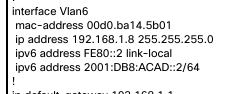
\includegraphics[width=0.6\linewidth]{images/run-conf-vlan}
	\caption{Запись о vlan 6 в текущем файле конфигурации}
	\label{fig:run-conf-vlan}
\end{figure}


Ограничим доступ к коммутатору по линиям консоли и vty, установив пароль cisco. Настроем локальную авторизацию на данных линиях командой \textit{login}, находясь в режиме конфигурации данных линий. 

Установим возможность удаленного соединения к коммутатору по протоколу Telnet, выполним команды \textit{transport input telnet}, находясь в режиме конфигурации линий vty.

\step{Настройте IP-адрес на компьютере PC-A}
{
Проведем аналогичные действия с PC-A. Настроим IPv4 и IPv6, шлюз по умолчанию 192.168.1.1, имитировав маршрутизатор (см. рисунок \ref{fig:pc-a-ip-settings}).

% TODO: \usepackage{graphicx} required
\begin{figure}[h!]
	\centering
	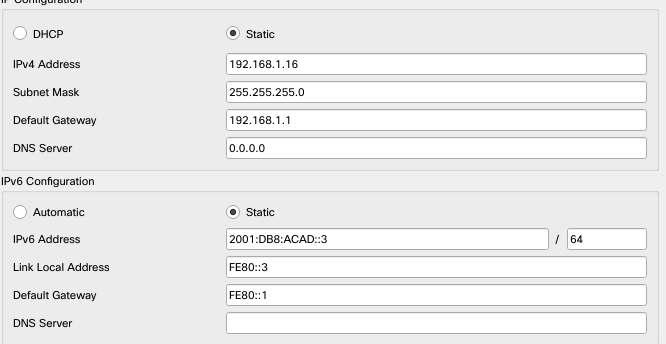
\includegraphics[width=0.6\linewidth]{images/pc-a-ip-settings}
	\caption{Сетевые настройки PC-A}
	\label{fig:pc-a-ip-settings}
\end{figure}
}

\mypart{Проверка сетевых подключений}
{
	
\step{Протестируйте сквозное соединение, отправив эхо-запрос}
Проверим сетевое соединение между устройствами (см. рисунок \ref{fig:switch-to-pc1}), отправив эхо-запрос на PC-A по адресу 192.168.1.16.

% TODO: \usepackage{graphicx} required
\begin{figure}[h!]
	\centering
	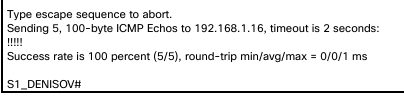
\includegraphics[width=0.6\linewidth]{images/switch-to-pc1}
	\caption{Эхо запрос к PC-A}
	\label{fig:switch-to-pc1}
\end{figure}





Проверим конфигурацию виртуального интерфейса vlan 6 с помощью команды \textit{show interface vlan6} (см. рисунок \ref{fig:show-interface-vlan6}).
% TODO: \usepackage{graphicx} required
\begin{figure}[h!]
	\centering
	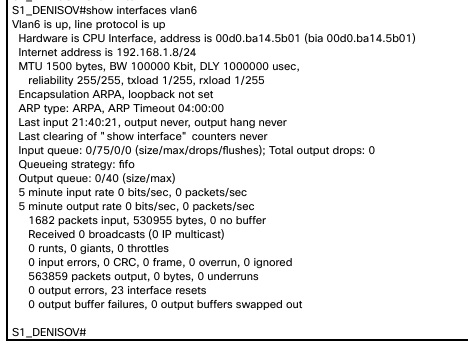
\includegraphics[width=0.6\linewidth]{images/show-interface-vlan6}
	\caption{Результат работы команды show interface vlan6}
	\label{fig:show-interface-vlan6}
\end{figure}

Полоса пропускания интерфейса Vlan 6 = 100 Mib/s. Vlan 6 находится во включенном состоянии.



}
\step{Проверьте удаленное управление коммутатором}

{
	Проверим удаленное подключение к коммутатору по протоколу Telnet, выполнив команду \textit{telnet 192.168.1.8} из терминала PC-A. В качестве пароля линии введем \textbf{cisco}. Для входа в привилегированный режим будем использовать пароль \textbf{class}. Результаты подключения приведены на рисунке \ref{fig:pc-to-swith}.
% TODO: \usepackage{graphicx} required
\begin{figure}[h!]
	\centering
	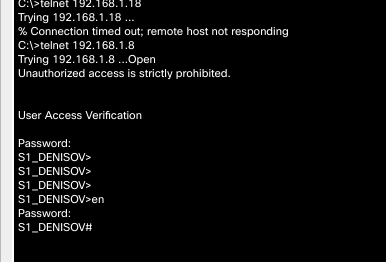
\includegraphics[width=0.6\linewidth]{images/pc-to-swith}
	\caption{Telnet подключение к коммутатору}
	\label{fig:pc-to-swith}
\end{figure}
}

\mypart{Управление таблицей MAC-адресов}
{
{
\step{Запишите MAC-адрес узла}{

Воспользуемся командой \textit{ipconfig /all}, чтобы узнать физический адрес сетевой интерфейсной платы PC-A. 	
Physical Address................: 000D.BDAA.C015
}
\step{Определите МАС-адреса, полученные коммутатором}
{
Воспользуемся командой \textit{show mac address-table} на коммутаторе, чтобы вывести таблицу известных MAC-адресов (см. рисунок \ref{fig:show-mac-address}). Как видим, это адрес узла PC-A.

% TODO: \usepackage{graphicx} required
\begin{figure}[h!]
	\centering
	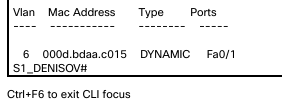
\includegraphics[width=0.7\linewidth]{images/show-mac-address}
	\caption{Таблица MAC-адресов на коммутаторе}
	\label{fig:show-mac-address}
\end{figure}

\step{Перечислите параметры команды show mac address-table}

Выведем параметры команды \textit{show mac address-table} (см. рисунок \ref)

% TODO: \usepackage{graphicx} required
\begin{figure}[h!]
	\centering
	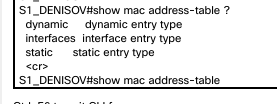
\includegraphics[width=0.6\linewidth]{images/show-mac-address-params}
	\caption{Параметры команды show mac address-table}
	\label{fig:show-mac-address-params}
\end{figure}

В данной таблице при использовании параметра dynamic мы видим только один адрес. 

\step{Назначьте статический MAC-адрес}

Назначим статический MAC-адрес предварительно очистив таблицу MAC-адресов командой \textit{clear mac address-table dynamic} (см. рисунок \ref{fig:clear-mac-table}).

% TODO: \usepackage{graphicx} required
\begin{figure}[h!]
	\centering
	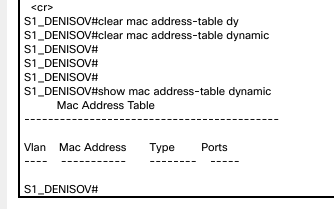
\includegraphics[width=0.7\linewidth]{images/clear-mac-table}
	\caption{Очистка таблицы MAC-адресов}
	\label{fig:clear-mac-table}
\end{figure}

Отравив эхо-запрос с узла PC-A обнаружим, что в таблицу снова попал физический адрес PC-A --- это говорит о работе протокола ARP.


Назначим статический адрес PC-A для интерфейса vlan 6 с помощью команды
\textit{\# mac address-table static 000D.BDAA.C015 vlan 6 interface fastethernet 0/6}. После этого в таблице MAC-адресов появится запись о том, что статический адрес добавлен (см. рисунок \ref{fig:static-mac}).


% TODO: \usepackage{graphicx} required
\begin{figure}
	\centering
	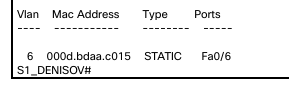
\includegraphics[width=0.7\linewidth]{images/static-mac}
	\caption{Добавление статического адреса}
	\label{fig:static-mac}
\end{figure}

}



}
}

\subsection*{Ответы на вопросы}
\begin{enumerate}
	\item Auto-MDIX
	Ethernet интерфейс Auto-MDIX способен автоматически определять какой вид порта требуется, при использовании Auto-MDIX тип используемого кабеля не имеет значения. Можно использовать как прямой, так и перекрестный кабель.
	
	\item SSH обеспечивает шифрование передаваемых и отправляемых данных, защищая данные от перехвата. Telnet не обеспечивает шифрование данных. При использовании данных подключений используется протокол TCP транспортного уровня. Порт SSH -- 22, Telnet -- 23.
	\item Данный интерфейс нужен для проверки отправки пакетов от устройства самому себе. Также данный интерфейс может быть зарезервирован для дальнейшего расширения сети. С помощью истории команд можно более быстро и продуктивно выполнять однотипные команды, а также позволяет увидеть, какие команды были запущены ранее. 
	\item В таблице содержится информация об известных сетевых и физических адресах устройств сети, которые были получены в результате работы протокола ARP. Также имеется информация о типе данных записей --- статическая или динамическая. Данные попадают в таблицу, после того, как устройства отзываются на ARP запрос от коммутатора, который посылается им периодически всем устройствам в сети.
	\item 
\end{enumerate}

\end{document}



